\documentclass{standalone}


\usepackage{tikz, pgfplots}
\usepgfplotslibrary{groupplots}
\pgfplotsset{compat=1.18} 
\usepgfplotslibrary{fillbetween}
\usepackage{graphicx}

\begin{document}
	
	\begin{tikzpicture}
		\node at (3,4){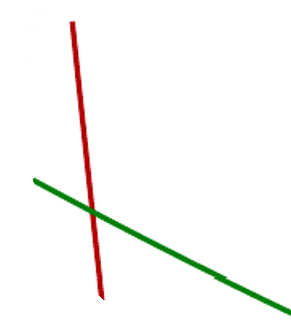
\includegraphics[scale=0.3]{Capture.png}};		
		\begin{axis}[
			%axis y line*=left,
			xmin = 0, xmax = 1.3,
			ymin=0, ymax=1.3,
			%legend style={at={(1.35,0.38)}},
			xlabel=$f_1$,
			ylabel=$f_2$,
			axis lines = left,
				xtick={0},
			ytick={0}
			];
			
	\addplot[color=red!70!black,smooth, domain=0.04:0.8]{0.03*(1/x)};
	\addplot[color=green!50!black,smooth, domain=0.02:0.95]{1/((1.5*e^x))};

\end{axis}
\node [draw,dashed,circle,scale=20,inner sep=0pt] at(0.35,3){};
\node [draw,dashed,circle,scale=60,inner sep=0pt] at(3.2,4){};
\draw[dashed] (0.71,3) --(1,3 );
\draw[-stealth,dashed] (1.05,3.02) --(2.1,4);


	\end{tikzpicture}
\end{document}